\documentclass{article}
\usepackage{tikz}
\usetikzlibrary{shapes.geometric, arrows, positioning}
\usepackage[margin=0.5cm]{geometry}

% Estilos
\tikzset{
    mybox/.style = {
        rectangle, 
        draw=blue!70!black, 
        fill=blue!10, 
        minimum width=3.8cm, 
        minimum height=1.2cm, 
        align=center,
        thick
    },
    mystart/.style = {
        rectangle, 
        rounded corners=10pt, 
        draw=green!70!black, 
        fill=green!15, 
        minimum width=3.8cm, 
        minimum height=1.2cm, 
        align=center,
        thick
    },
    myplugin/.style = {
        rectangle,
        draw=purple!70!black,
        fill=purple!10,
        minimum width=3.8cm,
        minimum height=1.2cm,
        align=center,
        thick,
        rounded corners=5pt
    },
    mystorage/.style = {
        cylinder, 
        draw=orange!70!black, 
        fill=orange!15, 
        shape border rotate=90, 
        minimum height=1.8cm, 
        minimum width=2.5cm, 
        aspect=0.25,
        thick
    },
    myoutput/.style = {
        rectangle,
        draw=red!70!black,
        fill=red!10,
        minimum width=3.8cm,
        minimum height=1.2cm,
        align=center,
        thick
    },
    myarrow/.style = {
        thick, 
        ->,
        >=stealth
    }
}

\begin{document}
\pagestyle{empty}
\begin{center}
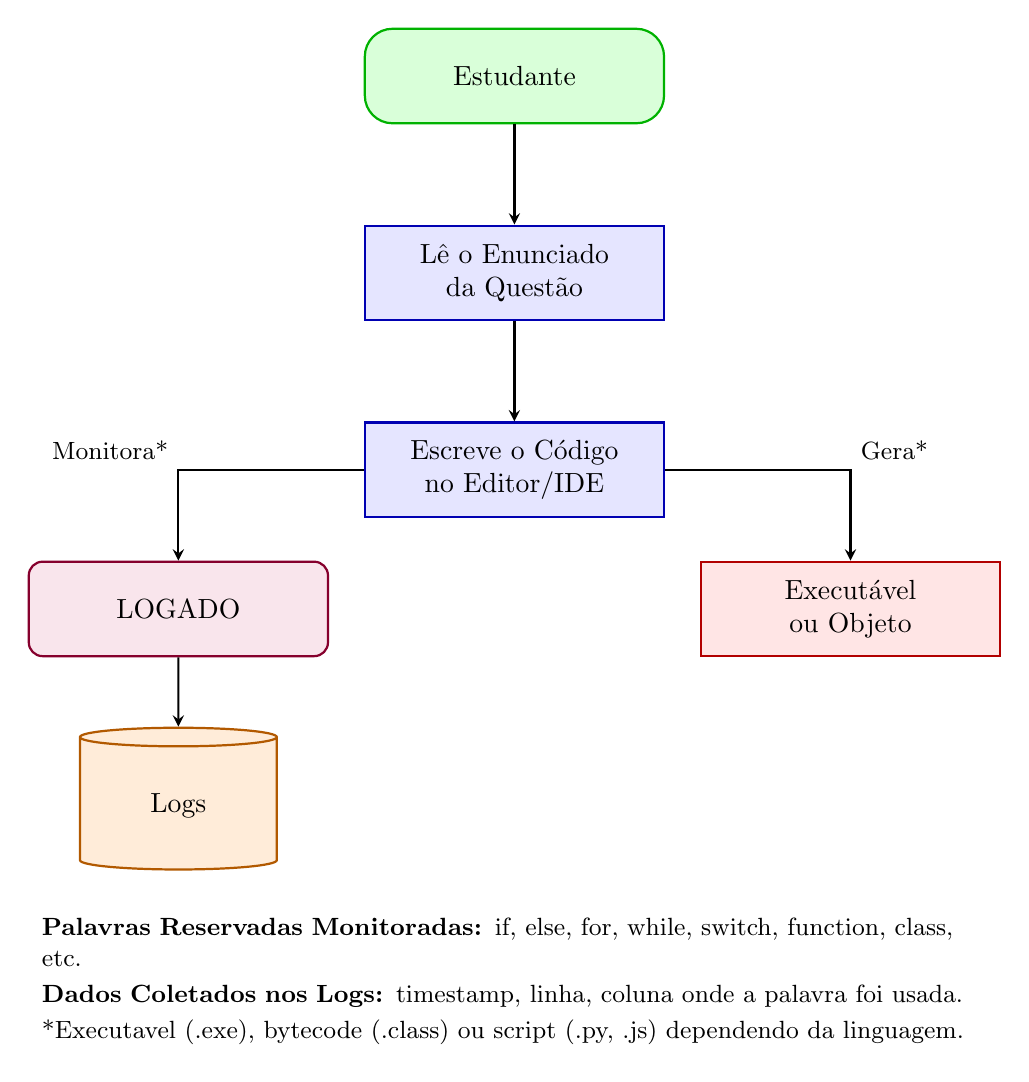
\begin{tikzpicture}[node distance=2.5cm]

% Definindo os nos
\node (estudante) [mystart] {Estudante};
\node (enunciado) [mybox, below of=estudante] {Lê o Enunciado\\da Questão};
\node (editor) [mybox, below of=enunciado] {Escreve o Código\\no Editor/IDE};
\node (plugin) [myplugin, below left of=editor, xshift=-2.5cm] {LOGADO};
\node (logs) [mystorage, below of=plugin] {Logs};
\node (executavel) [myoutput, below right of=editor, xshift=2.5cm] {Executável\\ou Objeto};

% Conectando com setas
\draw [myarrow] (estudante) -- (enunciado);
\draw [myarrow] (enunciado) -- (editor);

% Caminho do plugin (esquerda)
\draw [myarrow] (editor) -| (plugin) node[midway, above left, font=\small] {Monitora*};
\draw [myarrow] (plugin) -- (logs);

% Caminho do executavel (direita)
\draw [myarrow] (editor) -| (executavel) node[midway, above right, font=\small] {Gera*};

% Nota de rodape com palavras reservadas
\node [text width=12cm, below of=editor, yshift=-4cm, font=\small, align=left] {
    \textbf{Palavras Reservadas Monitoradas:} if, else, for, while, switch, function, class, etc.\\[2pt]
    \textbf{Dados Coletados nos Logs:} timestamp, linha, coluna onde a palavra foi usada.\\[2pt]
    *Executavel (.exe), bytecode (.class) ou script (.py, .js) dependendo da linguagem.
};

\end{tikzpicture}
\end{center}
\end{document}